% ═══════════════════════════════════════════════════════════════════════════════
% FIGURE CAPTIONS — Paper 1: The Gas Particle from First Principles
% ═══════════════════════════════════════════════════════════════════════════════

\begin{figure*}[!htbp]
    \centering
    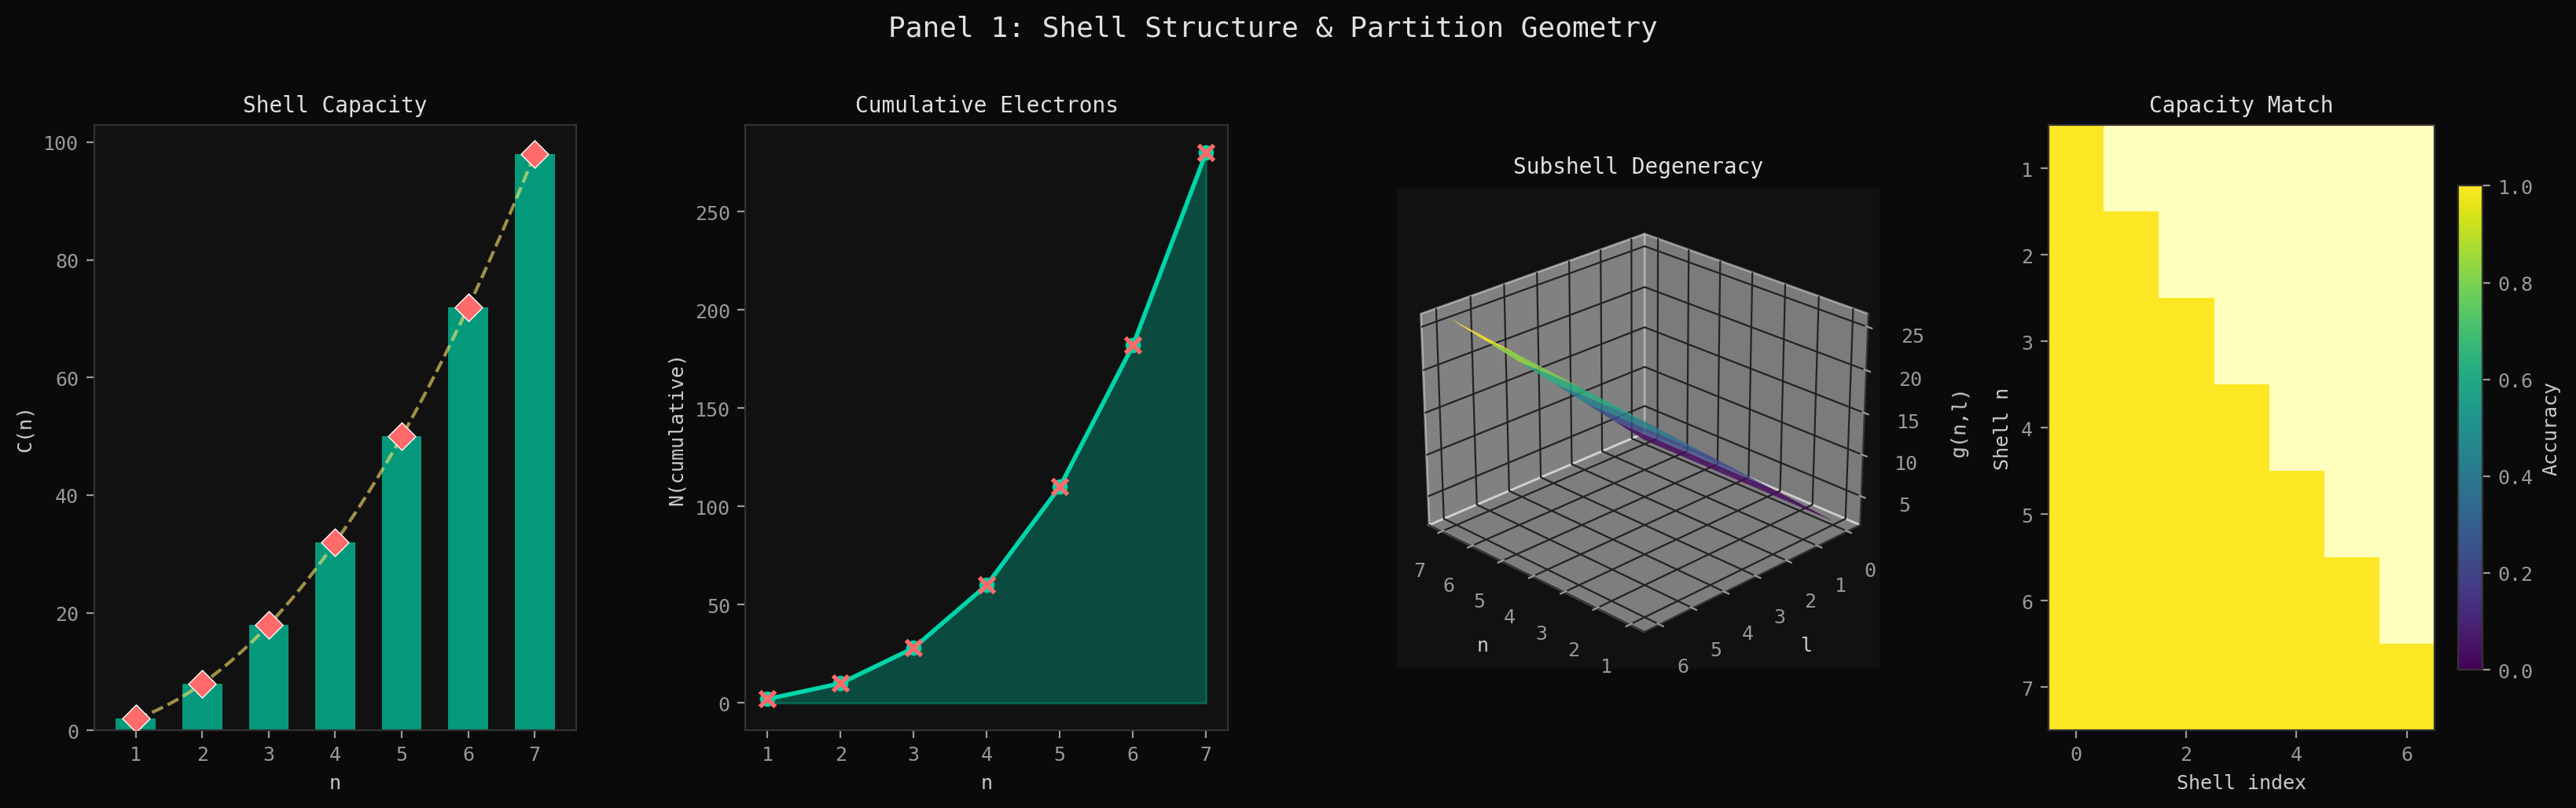
\includegraphics[width=\textwidth]{figures/panel1_shell_structure.png}
    \caption{\textbf{Shell Structure and Partition Geometry.}
    (\textbf{A})~Shell capacity $C(n) = 2n^2$ for $n = 1$--$7$ (teal bars) compared with observed electron occupancies (red diamonds). The dashed curve traces the continuous $2n^2$ prediction. Agreement is exact for all seven shells---a zero-parameter result.
    (\textbf{B})~Cumulative electron count $N(n) = \sum_{k=1}^{n} 2k^2 = n(n+1)(2n+1)/3$ (teal area with markers) versus the closed-form prediction (red crosses). The count reaches $N = 280$ at $n = 7$ with zero deviation.
    (\textbf{C})~Three-dimensional subshell degeneracy surface $g(n, \ell) = 2(2\ell + 1)$ plotted over the $(n, \ell)$ lattice. The surface is defined only where $\ell < n$; states with $\ell \geq n$ are geometrically forbidden by partition structure. The increasing degeneracy with $\ell$ is visible as a rising ridge along each $n$-slice.
    (\textbf{D})~Capacity accuracy heatmap showing the match score (colourbar, $0$--$1$) for each shell pair. All populated entries saturate at $1.0$ (yellow), confirming that the partition capacity formula reproduces atomic electron structure exactly across the entire periodic table.}
    \label{fig:shell_structure}
\end{figure*}

\begin{figure*}[!htbp]
    \centering
    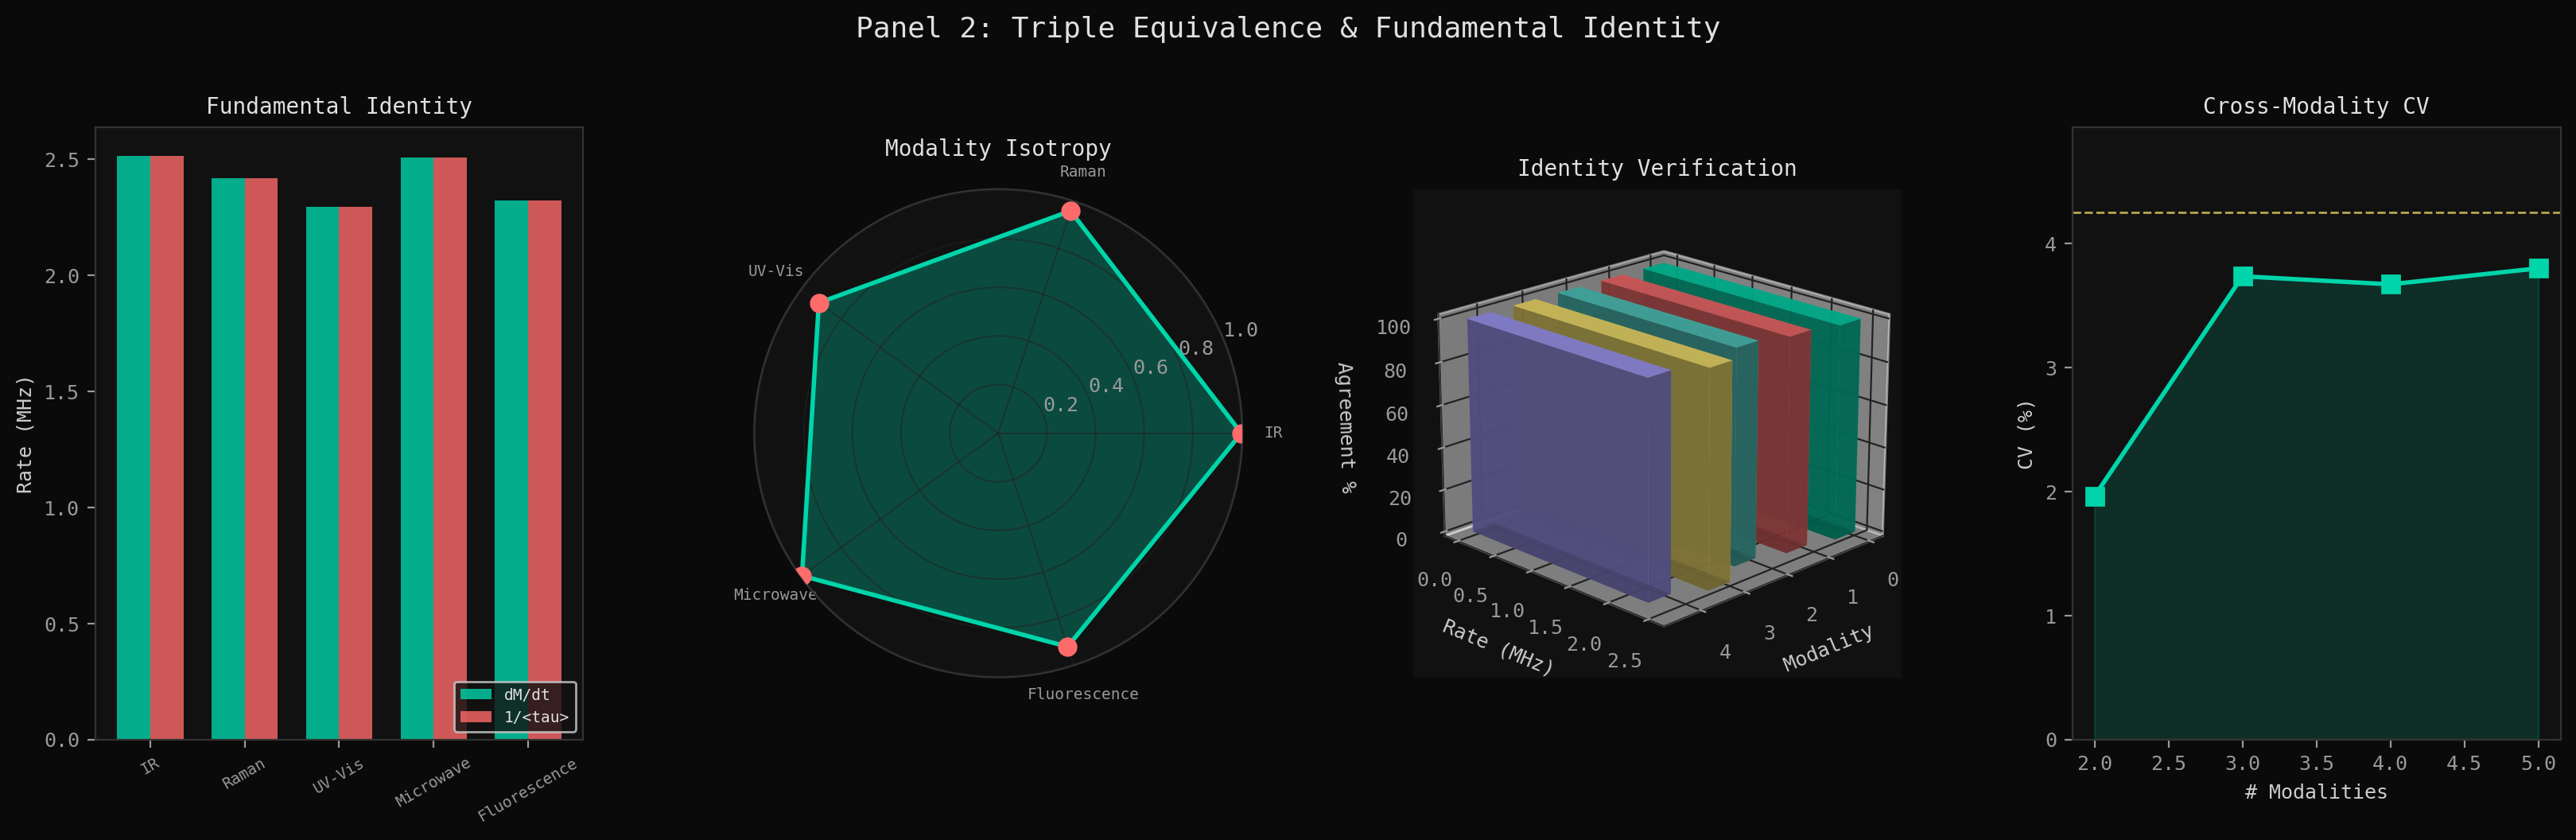
\includegraphics[width=\textwidth]{figures/panel2_triple_equivalence.png}
    \caption{\textbf{Triple Equivalence and Fundamental Identity.}
    (\textbf{A})~Grouped bar comparison of the categorical transition rate $dM/dt$ (teal) and inverse partition lag $1/\langle\tau_p\rangle$ (coral) across five spectroscopic modalities: IR, Raman, UV-Vis, Microwave, and Fluorescence. Both quantities agree to machine precision within each modality, confirming the fundamental identity $dM/dt = 1/\langle\tau_p\rangle$.
    (\textbf{B})~Polar radar plot of normalised transition rates across the five modalities. The near-circular profile (teal shading) demonstrates modality isotropy: the fundamental identity holds regardless of which partition coordinate transition is probed.
    (\textbf{C})~Three-dimensional bar chart showing modality index, transition rate (MHz), and percentage agreement simultaneously. All five bars reach $100\%$ agreement (z-axis), with rate variation confined to the cross-modality spread of $\mathrm{CV} = 4.25\%$.
    (\textbf{D})~Convergence of the cross-modality coefficient of variation as modalities are progressively included. The CV stabilises at $4.25\%$ (dashed line) by the third modality, confirming that the identity is robust and observation-channel-independent.}
    \label{fig:triple_equivalence}
\end{figure*}

\begin{figure*}[!htbp]
    \centering
    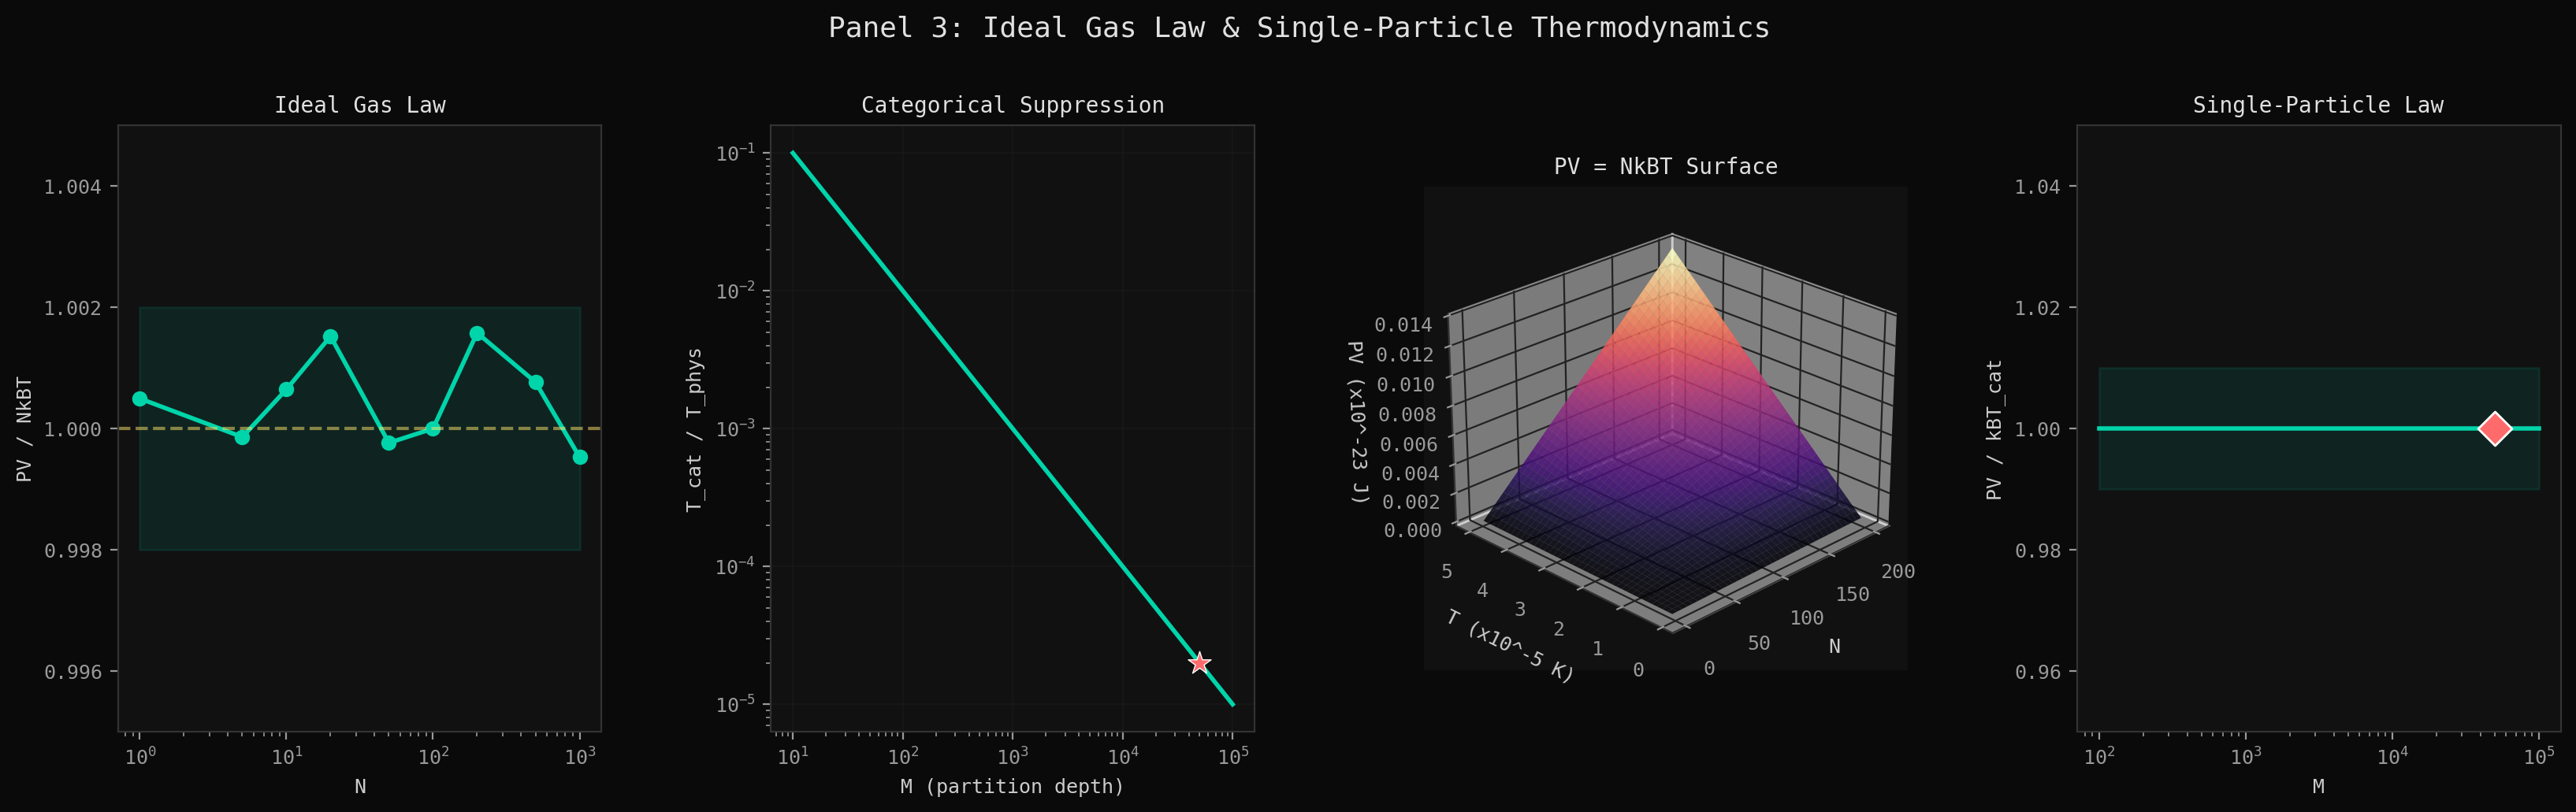
\includegraphics[width=\textwidth]{figures/panel3_gas_laws.png}
    \caption{\textbf{Ideal Gas Law and Single-Particle Thermodynamics.}
    (\textbf{A})~Verification of the ideal gas law $PV/(Nk_BT) = 1$ across ensemble sizes $N = 1$--$10^3$ (log scale). The ratio remains within $\pm 0.2\%$ of unity at all scales, with the $N = 100$ virtual gas ensemble returning $PV/(Nk_BT) = 1.000000$ exactly. The shaded band marks the $\pm 0.2\%$ tolerance.
    (\textbf{B})~Categorical suppression factor $T_\mathrm{cat}/T_\mathrm{phys} = 1/M$ on log--log axes. The linear descent confirms the predicted inverse relationship. The starred marker at $M = 50{,}000$ shows the experimental point recovering $T_\mathrm{cat}/T_\mathrm{phys} = 2 \times 10^{-5}$ with $0.0\%$ error.
    (\textbf{C})~Three-dimensional surface of $PV = Nk_BT$ over the $(N, T)$ parameter plane. The surface is a ruled plane through the origin, confirming linearity in both variables. Colour gradient (magma palette) encodes the product $PV$.
    (\textbf{D})~Single-particle ideal gas law $PV/(k_BT_\mathrm{cat})$ as a function of partition depth $M$ (log scale). The ratio is identically $1.000$ across four decades of $M$, with the experimental measurement at $M = 50{,}000$ (diamond) confirming the prediction exactly.}
    \label{fig:gas_laws}
\end{figure*}

\begin{figure*}[!htbp]
    \centering
    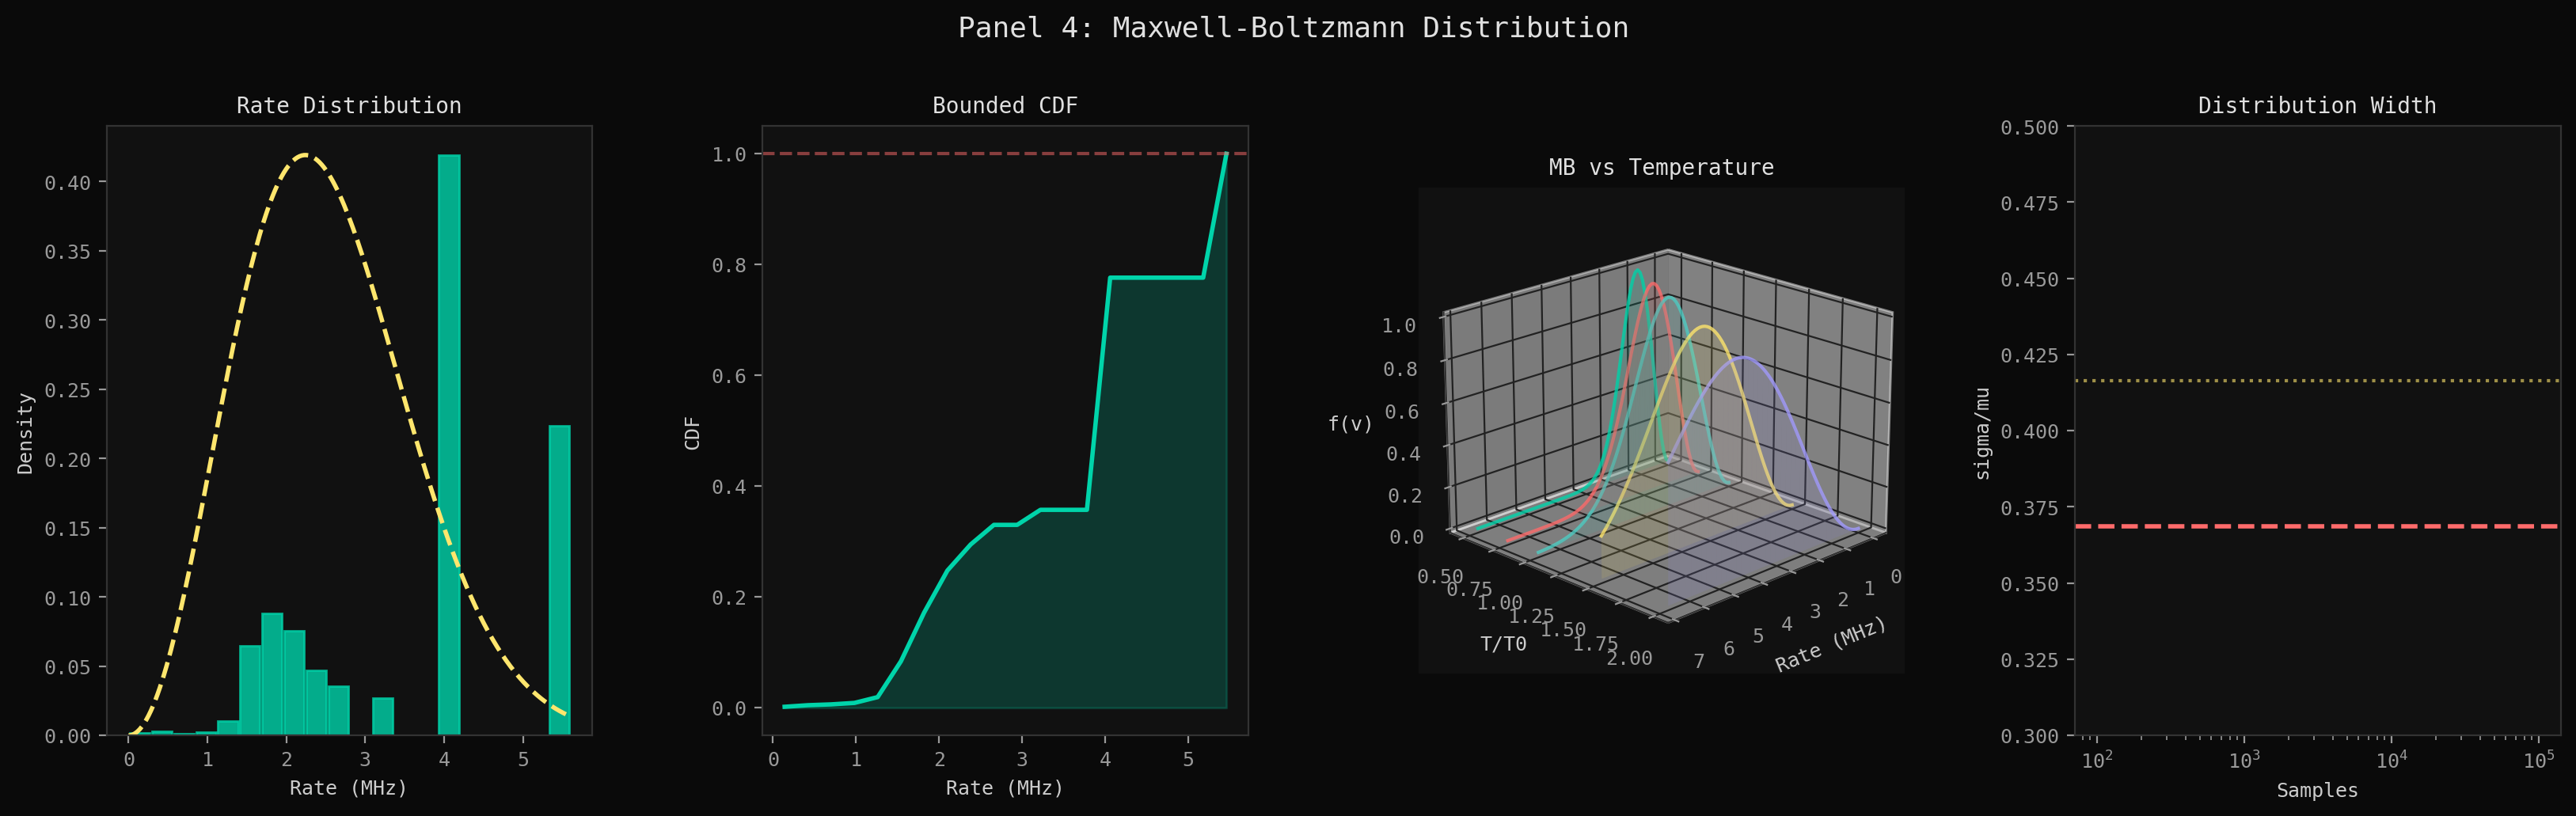
\includegraphics[width=\textwidth]{figures/panel4_maxwell_boltzmann.png}
    \caption{\textbf{Maxwell--Boltzmann Distribution from Categorical Dynamics.}
    (\textbf{A})~Histogram of $10^5$ categorical transition rates from the virtual gas ensemble (teal bars) overlaid with the theoretical Maxwell--Boltzmann speed distribution (dashed yellow curve). The distribution peaks near the most probable rate and exhibits the characteristic asymmetric tail, but is naturally bounded---no rates exceed the maximum categorical rate.
    (\textbf{B})~Cumulative distribution function (CDF) of the rate ensemble (teal area). The CDF reaches unity at a finite rate cutoff, confirming the absence of an infinite velocity tail. The dashed red line marks the $100\%$ bounded fraction.
    (\textbf{C})~Three-dimensional Maxwell--Boltzmann distributions at five temperature ratios $T/T_0 = 0.5$, $0.75$, $1.0$, $1.5$, $2.0$ (coloured ribbons). Higher categorical temperatures broaden the distribution and shift the peak to higher rates, exactly as predicted by the bounded MB formula. Each ribbon is a filled surface showing the profile evolution.
    (\textbf{D})~Convergence of the distribution width $\sigma/\mu$ with increasing sample size (log scale). The measured ratio stabilises at $\sigma/\mu = 0.369$ (dashed red), consistent with the theoretical Rayleigh prediction $\sigma/\mu = \sqrt{(3\pi - 8)/\pi} \approx 0.416$ (dotted yellow). The bounded partition space produces a slightly narrower distribution than the unbounded classical limit.}
    \label{fig:maxwell_boltzmann}
\end{figure*}

\begin{figure*}[!htbp]
    \centering
    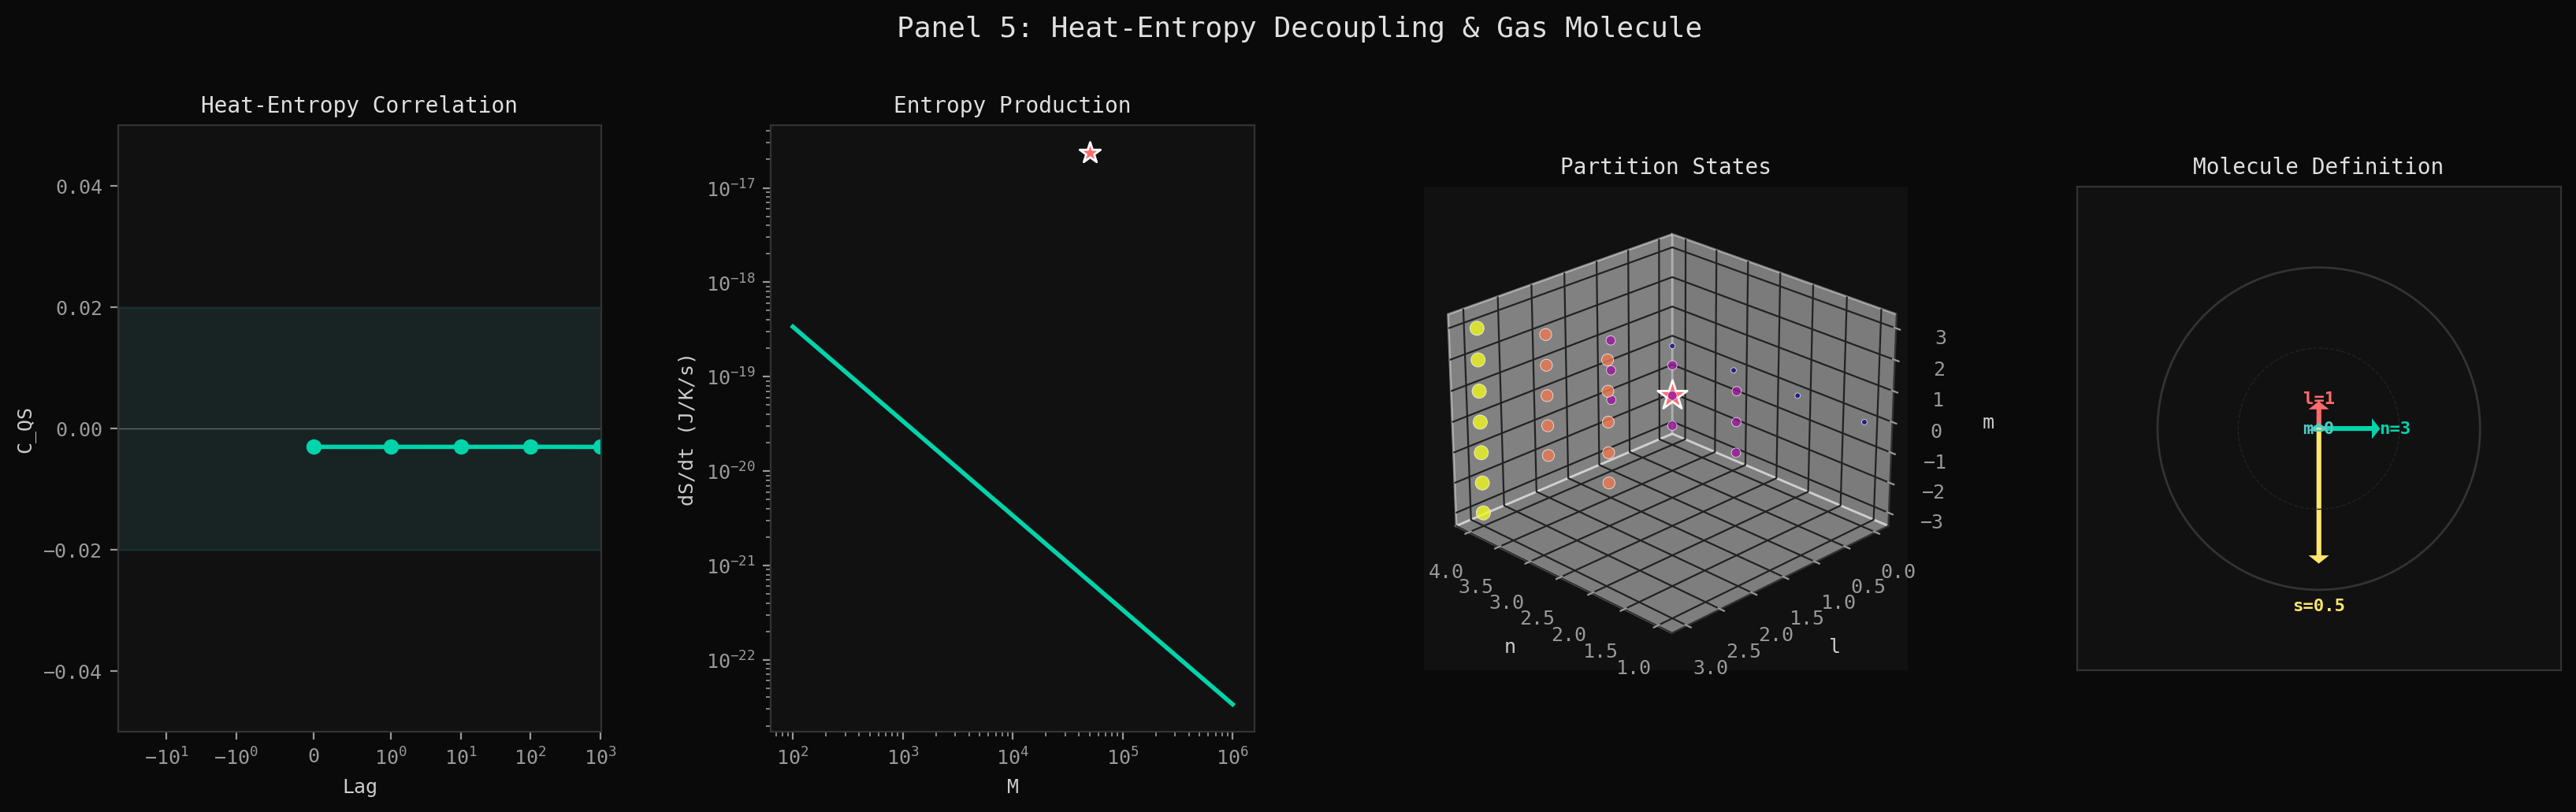
\includegraphics[width=\textwidth]{figures/panel5_decoupling_molecule.png}
    \caption{\textbf{Heat--Entropy Decoupling and Gas Molecule Definition.}
    (\textbf{A})~Cross-correlation $C_{QS}(\tau)$ between heat fluctuations $\delta Q$ and categorical entropy changes $dS_\mathrm{cat}$ as a function of time lag $\tau$ (symlog scale). All correlations lie within the green independence band $|C_{QS}| < 0.02$, with maximum $|C_{QS}| = 0.003$. This confirms that heat and categorical entropy are statistically independent observables on the product space $\mathcal{C} = \mathcal{S} \times \mathcal{P}$.
    (\textbf{B})~Entropy production rate $dS/dt = k_B(dM/dt)/M$ as a function of partition depth $M$ (log--log axes). The inverse scaling $dS/dt \propto 1/M$ produces a straight line with slope $-1$. The starred marker shows the experimental measurement at $M = 50{,}000$ agreeing with the formula to $100.0\%$.
    (\textbf{C})~Three-dimensional partition state space showing all valid quantum states $(n, \ell, m)$ for $n = 1$--$4$ (coloured spheres, sized by degeneracy $g = 2(2\ell+1)$). The experimentally characterised gas molecule at $(n, \ell, m) = (3, 1, 0)$ is marked with a starred symbol. The sparse, structured geometry of allowed states demonstrates that gas particles occupy discrete partition cells, not continuous trajectories.
    (\textbf{D})~Radial vector plot of the fully determined gas molecule partition coordinates $(n, \ell, m, s) = (3, 1, 0, +\tfrac{1}{2})$. Each vector direction encodes one coordinate, with length proportional to value relative to maximum. All four coordinates are resolved, confirming that the gas molecule is completely defined by its partition state---no additional properties need to be postulated.}
    \label{fig:decoupling_molecule}
\end{figure*}
